\documentclass[conference]{IEEEtran}
\IEEEoverridecommandlockouts
\usepackage{cite}
\usepackage{amsmath,amssymb}
\usepackage{graphicx}
\usepackage{textcomp}
\usepackage{hyperref}

\begin{document}

\title{Testing Physics Regularization for Event-Camera Vibration Estimation Under Sensing-Condition Shift}

\author{\IEEEauthorblockN{Arnab Mandal, Suryansh Rohil, and Shresth Tiwari}
\IEEEauthorblockA{Department of Computer Science and Engineering,\\
Shiv Nadar University\\
{\tt (am483, sr738, st637)@snu.edu.in}}
}

\maketitle

\begin{abstract}
Event cameras can observe structural vibration without contact at microsecond resolution, but it is unclear whether learned event-to-waveform estimators remain accurate when illumination or sensor settings change. We study this on 30 hammer-impact free-decay trials of an H-beam (XJTU-DV-Beam), grouped into six sensing conditions, with a laser Doppler vibrometer (LDV) as reference.

We define a robustness gap $\Delta$, the change in error between held-out and matched conditions, and a pre-specified falsification rule: a single-degree-of-freedom (SDOF) physics residual counts as helpful only if its $\Delta$ reduction exceeds trial-to-trial uncertainty. Using trial-level leave-one-condition-out evaluation, we compare a 3D-ResNet, a Kinetics-pretrained space-time Transformer, and a ridge regression baseline.

The physics term failed to clear noise on all six control folds, raised the matched-condition RMSE point estimate on most folds (not tested for significance), and showed a compute cost within timing noise. No model recovered waveform shape (Pearson $r \leq 0.24$ against a target above $0.9$). Deep models reached matched RMSE of 0.19--3.08 against a window-level zero-prediction RMSE of 1.71--2.05 on the same high-variance folds, while ridge regression reached 0.29--0.66 by capturing amplitude envelope only.

Probing showed that latents encode envelope decay but not natural frequency. Shifted conditions were often easier than matched ones, indicating that the matched reference is unstable at these sample sizes.

We contribute the $\Delta$ protocol, an event-to-LDV pipeline, a normalized-residual collapse guard, and a failure taxonomy that identifies ridge regression as a competitive baseline for future event-based vibration estimation.
\end{abstract}

\begin{IEEEkeywords}
event camera, non-contact vibration measurement, structural health monitoring (SHM), physics-informed learning, robustness gap
\end{IEEEkeywords}

\section{Introduction}
Vibration is the primary observable in structural health monitoring (SHM): changes in stiffness, mass or damping shift natural frequencies and reshape the dynamic response of bridges, beams, turbines and machinery. Each common sensing option has a drawback. Bonded accelerometers add mass and wiring and so alter the dynamics they measure. Laser Doppler vibrometers (LDVs) are accurate but need a stationary head and a clear line of sight. Frame cameras are contactless but blur on fast, small motion. A lower-cost, non-contact optical sensor that tolerates field lighting would ease inspection and continuous monitoring.

Event cameras are a candidate. Each pixel asynchronously reports a brightness change when $|\Delta \log I|$ exceeds a contrast threshold $C$, with microsecond timestamps and roughly 140~dB dynamic range, against about 60~dB for conventional CMOS sensors~\cite{Gallego2020,Rebecq2021}. These properties suit vibration measurement in principle. Recent work on event-based deformation measurement fuses events with co-registered frames and solves for dense displacement fields without training~\cite{Wu2026}.

That approach outputs deformation rather than an LDV-referenced waveform, requires a synchronised frame stream, is optimised separately for each sequence with no learned prior across recordings, depends on brightness constancy and spatial continuity, and was not evaluated under changes to the sensing configuration.

Two other literatures bear on the problem but, to our knowledge, have not been combined with event data. Physics-informed learning adds governing-equation residuals to data fitting~\cite{Raissi2019}, though a poorly specified residual can degrade accuracy~\cite{Karniadakis2021}; in structural dynamics they improve data efficiency where mass, damping and stiffness are known or finite-element-derived~\cite{Wang2024}. The closest vision-based example fuses accelerometer and frame-camera displacement under a physics loss~\cite{Wu2025}, but it inherits frame-camera blur on fast, small motion and applies the residual to the accelerometer channel rather than a high-bandwidth optical one. SHM research has also addressed environmental variation, but through classification under open-set domain adaptation~\cite{Zhou2024}, which does not carry over to a continuous waveform target. Its transferable lesson is that training and test data should differ by construction rather than by random split, which we adopt. Video transformers add a data constraint: they need pretraining to compete with convolutional models at small sample sizes~\cite{Bertasius2021}.

The sensor itself is a source of domain shift. The effective contrast threshold varies across pixels~\cite{Gallego2020}, and illumination and bias settings change event rates, so the same physical motion can produce different event streams. For waveform regression there is no standard definition of robustness to this shift, since classification accuracy does not apply. A single-degree-of-freedom (SDOF) free-decay residual is a natural candidate remedy. It constrains the output to a physically plausible form whatever the sensing configuration. With only tens of trials, however, the residual must be identified from the same scarce data, and it can reward trivial solutions.

This paper tests that remedy. We learn a mapping $f_\theta$ from an event stream $E_s$, captured under sensing configuration $s$, to the waveform $\hat{q}(t)$ that a co-located LDV would record, and we ask two questions.

\textbf{RQ1 (accuracy):} Under matched acquisition conditions, can learned event-to-waveform estimators recover the LDV waveform and its dominant frequency?

\textbf{RQ2 (stability):} Does an SDOF physics residual reduce the robustness gap $\Delta = M(\text{shifted}) - M(\text{matched})$, with $M \in \{\text{RMSE, relative frequency error}\}$, by more than trial-to-trial uncertainty?

RQ2 is stated as a hypothesis with a pre-specified falsification rule: if the $\Delta$ reduction does not exceed its standard error, the physics term is reported as non-identifiable. A negative result is an admissible outcome.

Scope. The study uses 30 hammer-impact free-decay trials of one H-beam rig (XJTU-DV-Beam~\cite{Li2026}), grouped into six lighting/set conditions. The LDV reference is sampled at 256~Hz and the dominant mode lies near 6.7~Hz, so the sensor's kilohertz capability is not exercised here. We make no claim about damage classification or other structures.

Our contributions are: (1)~a continuous-waveform robustness protocol: the gap $\Delta$ with group-mean standard errors, trial-level leave-one-condition-out splits, and a falsification rule for regularisers; (2)~an event-to-LDV estimation pipeline (Struct-X) with a normalised-residual guard against the collapse $\hat{q} \to 0$ under scarce data; (3)~an empirical test across a 3D-ResNet, a Kinetics-pretrained divided space-time Transformer and a ridge baseline: the physics term fails to clear noise on all six control folds and raises the matched RMSE point estimate on most folds, and no model recovers waveform shape; (4)~a failure taxonomy, supported by latent probing, that identifies ridge regression as a competitive baseline for future work.

The remainder of the paper is organised as follows: Section~II describes the methods, Section~III the results and discussion, and Section~IV concludes.

\section{Methods}
\subsection{Problem Definition and Terminology}
Let $E_s = \{(x_i, y_i, t_i, p_i)\}$ be an asynchronous event stream with timestamps $t_i$ in microseconds and polarity $p_i \in \{-1, +1\}$, captured under sensing configuration $s$ (illumination, contrast threshold $C$, bias currents, sensor pose). Let $q(t)$ be the displacement recorded by a co-located LDV. We learn
\begin{equation}
\hat{q} = f_\theta(E_s), \quad \hat{q} \in \mathbb{R}^T,
\label{eq:map}
\end{equation}
together with a dominant-frequency estimate $\hat{f}_n$. A condition is one lighting/set combination (On or Off $\times$ set 1--3), giving six conditions. In each fold, one condition is held out as the shift condition. The remaining five conditions are the matched conditions, used for training and for matched evaluation.

\subsection{Data}
We use the Beam subset of XJTU-DV~\cite{Li2026,XJTU-DV-Beam}: 30 hammer-impact free-decay trials of an H-beam, five per condition, with event streams in Prophese-style \texttt{.dat} files and LDV velocity in \texttt{.txt} files. Sensor resolution ($1280\times720$) is read from the file headers. One event file carries a naming typo in the archive, which the pairing code handles. The LDV signal is sampled at 256~Hz, so it is integrated once to displacement and linearly detrended.

Event preprocessing. For each trial we (i)~mask hot pixels (event count above $5\times$ the median), (ii)~drop same-pixel events less than 100~$\mu$s apart, (iii)~crop to the contiguous y-band where the mean event count is at least 50\% of its peak, plus 8~px padding, and (iv)~build a voxel grid with $B = 5$ temporal bins and two polarity channels~\cite{Gallego2020}, giving a $(10, H, W)$ tensor. The longest side is resized to 224~px and zero-padded to a square, preserving aspect ratio. Each channel is standardised with a mean and standard deviation frozen from training trials only ($\epsilon = 10^{-6}$).

Target preprocessing. The displacement is low-pass filtered (4th-order Butterworth, 500~Hz), resampled to 1~kHz, and z-scored with frozen training statistics. Because the native rate is 256~Hz, the 500~Hz filter has no effect and the resampling is interpolation, so the effective bandwidth is 128~Hz. The dominant mode is near 6.7~Hz, giving 6--7 cycles per window. The frequency target $f_n$ is the FFT peak of the full LDV trial (Hann window, $4\times$ zero-padding, parabolic interpolation; search 5--500~Hz).

Windowing. Windows are 1.0~s long ($T = 1000$ samples) with a 0.5~s stride, anchored at the hammer trigger, taken as the peak of $|$velocity$|$ (argmax, no hardware trigger). Windows starting less than 100~ms after the trigger are excluded, because the physics model assumes free decay. This gives 326 windows. A synthetic threshold sweep with v2e~\cite{Hu2021} was explored as augmentation-grade only and is not part of the reported results.

\subsection{Split and Evaluation Protocol}
Splits are made at trial level only; window-level splitting is not used. We use leave-one-condition-out evaluation with $K = 6$ folds. In each fold, the five trials of the held-out condition form the shift set, and the 25 trials of the other five conditions form the matched pool. The matched pool is shuffled and split 15/5/5 into train, validation-matched and test-matched. The shift trials are split 2/3 into validation-shift (tuning and early stopping only) and test-shift (final reporting only). The seed is fixed at 0, and a leakage check confirms that no trial appears in two sets. Each fold therefore yields one $\Delta$, comparing five matched test trials with three shift test trials.

Metrics. Let $q_w[n]$ and $\hat{q}_w[n]$, $n=1\ldots T$, be the reference and estimate on test window $w$ ($T = 1000$, z-scored units), with window means $\bar{q}_w$ and $\bar{\hat{q}}_w$. Per-window metrics are
\begin{align}
\mathrm{RMSE}_w &= \sqrt{(1/T)\textstyle\sum_n (\hat{q}_w[n] - q_w[n])^2} \label{eq:rmse}\\
\mathrm{MAE}_w &= (1/T)\textstyle\sum_n |\hat{q}_w[n] - q_w[n]| \label{eq:mae}\\
r_w &= \frac{\sum_n (\hat{q}_w[n]-\bar{\hat{q}}_w)(q_w[n]-\bar{q}_w)}{\sqrt{\sum_n(\hat{q}_w[n]-\bar{\hat{q}}_w)^2 \cdot \sum_n(q_w[n]-\bar{q}_w)^2}} \label{eq:r}\\
\varepsilon_{f,w} &= |\hat{f}_{n,w} - f_n| / f_n \label{eq:freq}
\end{align}
We also record the normalised residual $\Phi_w = L_{\mathrm{phys}}$ (Eq.~\ref{eq:lphys}) evaluated on $\hat{q}_w$ as a self-consistency score. Pearson $r$ is computed per window and never pooled across windows. By implementation, $r_w = 0$ when either signal is constant, so a collapsed model has $r = 0$ rather than an undefined value. For trial $j$ with window set $W_j$, the trial-level value is
\begin{equation}
M_j = (1/|W_j|)\textstyle\sum_{w \in W_j} M_w. \label{eq:trial}
\end{equation}
The trial is the unit of analysis. All means, standard deviations and standard errors are taken over trials, never over windows. For a group $g$ of $n_g$ test trials, $\bar{M}_g = (1/n_g)\sum_j M_j$ and $s_g^2 = (1/(n_g-1))\sum_j (M_j - \bar{M}_g)^2$. Tuning and early stopping use a pooled-window RMSE on validation trials only, not the trial-level metric above.

Robustness gap. Trials are not paired across conditions, so $\Delta$ is a difference of group means:
\begin{align}
\Delta_M &= \bar{M}_{\mathrm{shift}} - \bar{M}_{\mathrm{matched}}, \quad M \in \{\mathrm{RMSE}, \mathrm{MAE}, \varepsilon_f\} \label{eq:delta}\\
\Delta_r &= \bar{r}_{\mathrm{matched}} - \bar{r}_{\mathrm{shift}} \label{eq:deltar}
\end{align}
with $\mathrm{se}_\Delta = \sqrt{s^2_{\mathrm{shift}}/n_{\mathrm{shift}} + s^2_{\mathrm{matched}}/n_{\mathrm{matched}}}$. The sign of $\Delta_r$ is reversed so that a positive $\Delta$ always means degradation. A negative $\Delta$ means the held-out condition scored better than the matched pool.

Pre-specified rule. For a given $M$, with ``base'' the data-only model and ``phys'' the physics-trained model,
\begin{equation}
R = \Delta_{\mathrm{base}} - \Delta_{\mathrm{phys}}, \quad \sigma_R = \sqrt{\mathrm{se}_{\mathrm{base}}^2 + \mathrm{se}_{\mathrm{phys}}^2}. \label{eq:o5}
\end{equation}
The physics term is declared helpful only if $R > \sigma_R$. Otherwise it is reported as non-identifiable. A result that fails this test is reported as failing to clear noise, never as evidence of equivalence. Matched-condition accuracy is reported separately as the difference in matched means. For RQ2's frequency comparison we compare $|\Delta_{\varepsilon_f}|$ with $|\Delta_{\mathrm{RMSE}}|$. The two quantities have different units, so this comparison is indicative only.

Zero-prediction reference. A model outputting $\hat{q} \equiv 0$ has an RMSE equal to the root-mean-square of the reference window. On the three high-variance folds a zero prediction scores a window-level RMSE of 1.71--2.05 (group mean over matched test trials).

\subsection{Models}
Encoders. Each takes the voxel tensor as $T = B$ frames with $C = 2$ channels and feeds a waveform head ($T = 1000$ outputs) and a frequency head (softplus output).
3D-ResNet18~\cite{He2016}: the 3-channel stem is converted to 2 channels by channel averaging.
TimeSformer~\cite{Bertasius2021}: divided space-time attention only (joint attention is excluded for memory), initialised from Kinetics-400 weights~\cite{Kay2017} with a 2-channel stem adaptation and temporal position embeddings interpolated to $B$ frames. The readout is a mean over patch tokens. The code is CC BY-NC 4.0, so this arm is research use only.
Ridge baseline: RidgeCV~\cite{Pedregosa2011} on per-channel temporal-bin means of the voxel grid (10 features, spatially averaged), fitted on training-trial windows only.

Loss. The total loss is
\begin{equation}
L = L_{\mathrm{LDV}} + \lambda_p \cdot L_{\mathrm{phys}} + \lambda_s \cdot L_{\mathrm{smooth}} + \lambda_f \cdot L_{\mathrm{freq}}, \quad \lambda_f = 0.1\ \mathrm{fixed} \label{eq:loss}
\end{equation}
with $L_{\mathrm{LDV}} = \mathrm{mean}_T \lVert \hat{q} - q \rVert^2$, $L_{\mathrm{smooth}} = \mathrm{mean}_T \lVert d\hat{q}/dt \rVert^2$ and $L_{\mathrm{freq}} = (\hat{f}_n - f_n)^2/f_n^2$. The SDOF residual is
\begin{equation}
L_{\mathrm{phys}} = \mathrm{mean}_T \lVert \hat{q}'' + c\,\hat{q}' + k\,\hat{q} \rVert^2 \,/\, (\mathrm{mean}_T \lVert \hat{q} \rVert^2 + \epsilon) \label{eq:lphys}
\end{equation}
with $m = 1$ by convention, because log-decrement fitting identifies only frequency and damping ratio. The denominator guards against the collapse $\hat{q} \to 0$, which would otherwise minimise the residual trivially. It makes $L_{\mathrm{phys}}$ amplitude-blind by design, so amplitude is set by $L_{\mathrm{LDV}}$ alone. Derivatives use second-order central differences in the interior and first-order one-sided differences at the endpoints, computed in fp32 with $\epsilon = 10^{-6}$.

Identifying $k$ and $c$. From one training trial per fold we estimate $\zeta$ by log decrement and the damped frequency $f_d$ from the spectrum. Then $f_n = f_d/\sqrt{1 - \zeta^2}$, $k = (2\pi f_n)^2$ and $c = 2\zeta\sqrt{k}$. Across folds $f_d \approx 6.7$~Hz, $k \approx 1800$ and $c \approx 2.2$--$2.9$. These values are frozen, and no validation, test or shift trial is used.

Ablation. Four variants are trained: (a)~data only, (b)~smoothness only, (c)~SDOF only, (d)~both. Each physics-bearing variant selects $(\lambda_p, \lambda_s)$ from the same $3\times3$ grid ($\lambda_p \in [10^{-3}, 10^{-1}]$, $\lambda_s \in [10^{-4}, 10^{-2}]$) by validation $\Delta_{\mathrm{RMSE}}$, with the same epoch budget. The frequency estimate $\hat{f}_n$ is the output of the trained head. The FFT peak of $\hat{q}$ is not used in reporting.

\subsection{Training and Implementation}
We use Adam (learning rate $2\times10^{-4}$), micro-batch 8 with gradient accumulation to an effective batch of 16, at most 50 epochs, and early stopping with patience 10 on validation $\Delta_{\mathrm{RMSE}}$. A gradient-ratio controller tracks $r = \lVert\nabla L_{\mathrm{phys}}\rVert/\lVert\nabla L_{\mathrm{LDV}}\rVert$. It scales $\lambda_p$ by 0.1 for the first five epochs, then halves $\lambda_p$ if $r > 1$ for three consecutive epochs and doubles it if $r < 0.01$ for three consecutive epochs, within $10^{-4}$ to $0.1$. Training is in full fp32. The ResNet control ran on an NVIDIA T4 and the pretrained arm on an RTX 4500 Ada. Latency is measured at batch size 1 on an input of shape $(1, 2, 5, 224, 224)$, with one warm-up pass, 20 timed passes and explicit CUDA synchronisation. Measured latency is 4--10~ms per window for the ResNet (load-dependent) and 42~ms for the TimeSformer on an RTX 4500 Ada at batch size 1, within the 50~ms budget.

Code and data availability. Code: \url{https://github.com/arnabwithab/struct-x} (tag \texttt{frozen-2026-11-04}). Data: Zenodo record 17447083, version v1, CC-BY-4.0. Kaggle: public dataset \texttt{eros483/struct-x-beam}; public kernels \texttt{eros438/struct-x-train}. Licence: MIT for code; the TimeSformer arm is CC BY-NC 4.0 and research-only.

\section{Results and Discussion}
\subsection{Matched accuracy (RQ1)}
Table~I gives the ResNet control results on all six folds for all four variants. Fold labels name the held-out (shift) condition. Each cell is matched RMSE $\pm$ trial std over the five matched test trials, with $\Delta_{\mathrm{RMSE}}$ in parentheses from the three shift test trials. Units are z-scored displacement.
\begin{table*}[t]
\caption{Matched RMSE ($\Delta_{\mathrm{RMSE}}$), 3D-ResNet control. (a)~data only, (b)~smoothness only, (c)~SDOF only, (d)~both.}
\label{tab:resnet}
\centering
\begin{tabular}{lcccc}
\hline
Fold & (a) & (b) & (c) & (d) \\
\hline
On\_set1 & 1.98$\pm$3.10 ($-$1.65) & 1.86$\pm$3.12 ($-$1.41) & 2.38$\pm$2.86 ($-$1.61) & 2.39$\pm$2.85 ($-$1.61) \\
Off\_set1 & 1.95$\pm$2.80 ($-$1.49) & 1.79$\pm$2.88 ($-$1.41) & 2.34$\pm$2.57 ($-$1.33) & 2.39$\pm$2.55 ($-$1.33) \\
Off\_set2 & 2.43$\pm$3.43 ($-$1.79) & 3.08$\pm$3.10 ($-$2.14) & 2.29$\pm$3.29 ($-$1.59) & 2.53$\pm$3.21 ($-$1.58) \\
Off\_set3 & 0.37$\pm$0.07 ($-$0.07) & 0.34$\pm$0.10 ($-$0.06) & 0.64$\pm$0.11 ($-$0.01) & 0.63$\pm$0.10 ($-$0.02) \\
On\_set2 & 0.52$\pm$0.10 ($+$2.23) & 0.43$\pm$0.17 ($+$2.23) & 1.05$\pm$0.25 ($+$1.94) & 0.99$\pm$0.21 ($+$1.98) \\
On\_set3 & 0.47$\pm$0.10 ($-$0.23) & 0.19$\pm$0.03 ($+$0.00) & 0.38$\pm$0.09 ($+$0.23) & 0.37$\pm$0.07 ($+$0.20) \\
\hline
\end{tabular}
\end{table*}

On the three high-variance folds (On\_set1, Off\_set1, Off\_set2), data-only matched RMSE is 1.95--2.43 -- at or worse than predicting nothing on the same windows (window-level zero RMSE 1.71--2.05). Trial stds of 2.8--3.4 on five trials imply at least one test trial with a very large error. Per-trial matched RMSE confirms it: one trial per fold scores 6.9--8.5 (On\_set1 7.5, Off\_set1 6.9, Off\_set2 8.5) with all others at or below 1.6, identically for data-only and both -- the same hard trial inflates every variant. On the other three folds, matched RMSE is 0.37--0.52, but Pearson $r$ is only 0.03--0.19. The gain over zero is therefore in amplitude, not waveform shape. The $r > 0.9$ target was missed by roughly a factor of five.

Matched RMSE varies more across folds than across training variants (Fig.~\ref{fig:matched}). Each fold's matched test set is five of 25 pooled trials, and the split is identical across variants (fixed seed). Fold-to-fold differences therefore plausibly reflect which trials land in test, and a single hard trial may inflate every variant on the high-variance folds.

\begin{figure}[t]
\centering
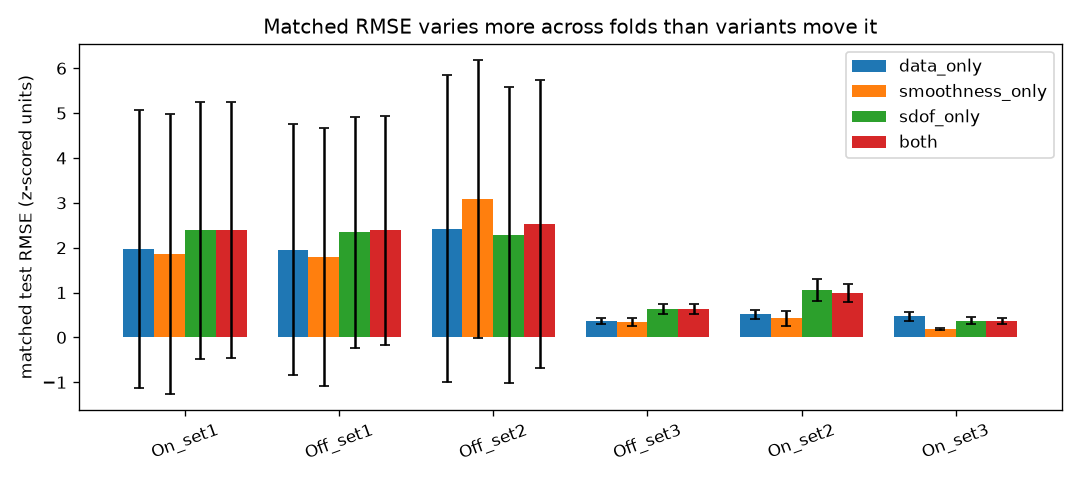
\includegraphics[width=\columnwidth]{figs/matched_rmse.png}
\caption{Matched test RMSE (mean $\pm$ trial std) by fold and variant. Variant (b) is smoothness-only.}
\label{fig:matched}
\end{figure}

\begin{table*}[t]
\caption{RidgeCV baseline. Matched is mean $\pm$ trial std; Pearson $r$ is matched.}
\label{tab:ridge}
\centering
\begin{tabular}{lcccc}
\hline
Fold & Matched RMSE & Shift RMSE & $\Delta_{\mathrm{RMSE}}$ & $r$ (matched) \\
\hline
On\_set1 & 0.657$\pm$0.713 & 0.303 & $-$0.354 & 0.198$\pm$0.127 \\
Off\_set1 & 0.499$\pm$0.512 & 0.322 & $-$0.178 & 0.201$\pm$0.068 \\
Off\_set2 & 0.637$\pm$0.638 & 0.274 & $-$0.363 & 0.171$\pm$0.084 \\
Off\_set3 & 0.389$\pm$0.098 & 0.631 & $+$0.242 & 0.240$\pm$0.126 \\
On\_set2 & 0.398$\pm$0.148 & 0.763 & $+$0.365 & 0.183$\pm$0.036 \\
On\_set3 & 0.292$\pm$0.067 & 0.358 & $+$0.066 & 0.232$\pm$0.044 \\
\hline
\end{tabular}
\end{table*}

Ridge regression on pooled voxel means reaches matched RMSE 0.29--0.66 and $r = 0.17$--$0.24$, with $|\Delta| \leq 0.37$. On the three high-variance folds it is far below every deep variant (0.50--0.66 against 1.8--3.1). On the other three folds the comparison is a near tie. Ridge (0.39, 0.40, 0.29) sits beside data-only (0.37, 0.52, 0.47) and smoothness-only (0.34, 0.43, 0.19) point estimates, with deep data-only marginally lower on Off\_set3. With $r \approx 0.2$, ridge captures the amplitude envelope and not the shape. In answer to RQ1, no model recovered the LDV waveform under matched conditions. A linear map on pooled voxel features is competitive with or better than every deep variant we trained. Per-trial Pearson $r$ for (b) is $-0.00$, 0.17, 0.14, 0.24, 0.14 and 0.25 across folds (On\_set1, Off\_set1, Off\_set2, Off\_set3, On\_set2, On\_set3) -- no shape recovery.

\subsection{Physics residual and the robustness gap (RQ2)}
Sign of $\Delta$. For data-only, $\Delta_{\mathrm{RMSE}}$ is negative on five of six folds (Table~I). The held-out condition scored better than the matched pool. We read this as a property of the benchmark. The matched reference is a five-trial mean that mixes five conditions with outlier trials, while each shift set is a single condition. Ridge shows mixed signs (three negative, three positive), and On\_set2 is positive for both ridge ($+$0.37) and deep ($+$2.23). That fold may be a genuinely harder condition, but its $\sigma_R$ of about 3 leaves it unresolved.

\begin{figure}[t]
\centering
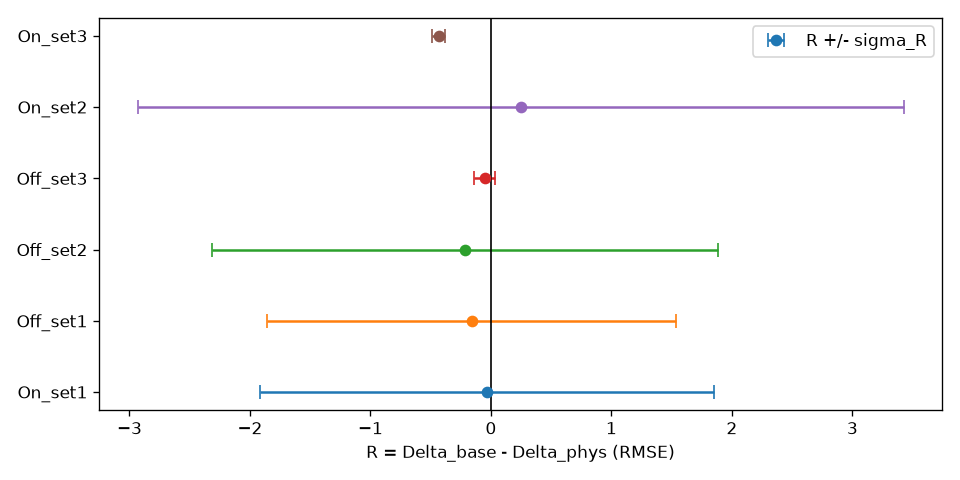
\includegraphics[width=\columnwidth]{figs/o5_forest.png}
\caption{$R = \Delta(a) - \Delta(d)$ (RMSE) with $\pm\sigma_R$, one point per fold. Physics counts as helpful only if the point lies beyond its bar on the positive side.}
\label{fig:o5}
\end{figure}

Falsification rule. Physics failed to clear noise on all six control folds (Fig.~\ref{fig:o5}). Table~\ref{tab:o5} gives the same test for (c) against (a). The (d)-against-(a) values for the three folds quoted exactly are Off\_set1 $R = -0.160$ ($\sigma_R$ 1.70), On\_set2 $+0.247$ (3.18) and On\_set3 $-0.434$ (0.056).
\begin{table}[t]
\caption{O5 test, SDOF only (c) against data only (a), RMSE.}
\label{tab:o5}
\centering
\begin{tabular}{lccc}
\hline
Fold & $R = \Delta(a) - \Delta(c)$ & $\sigma_R$ & Clears noise? \\
\hline
On\_set1 & $-0.037$ & 1.886 & No \\
Off\_set1 & $-0.159$ & 1.704 & No \\
Off\_set2 & $-0.200$ & 2.128 & No \\
Off\_set3 & $-0.062$ & 0.087 & No \\
On\_set2 & $+0.295$ & 3.163 & No \\
On\_set3 & $-0.463$ & 0.059 & No (harmful side) \\
\hline
\end{tabular}
\end{table}

On four folds $\sigma_R$ is 1.7--3.2 RMSE units, so those tests could not detect any plausible effect. The two folds with tight $\sigma_R$ (Off\_set3, On\_set3) are the ones that could resolve one. On On\_set3 the interval excludes zero on the harmful side for both (c) and (d). Physics raised the shifted RMSE from about 0.24 for (a) to about 0.61 for (c) and 0.57 for (d), while slightly lowering matched RMSE. We therefore report failure to clear noise, not equivalence. Note that the rule tests only for benefit, so the On\_set3 result is a descriptive observation about direction.

Matched-condition price. Relative to (a), (d) raised the matched RMSE point estimate on five of six folds, by 0.10--0.47, and (c) did so on four of six folds, by 0.27--0.53. On On\_set3 both lowered it by about 0.1, and (c) also lowered it on Off\_set2. On the three high-variance folds the changes lie far inside trial spread (std 2.6--3.4). On Off\_set3 and On\_set2 the increases of 0.26--0.53 exceed the trial std (0.07--0.25). No noise test was run on this quantity, so we call it a consistent but untested price, not a demonstrated harm.

Smoothness only. Variant (b) was trained on every fold. Its matched RMSE point estimate is below (a) on five of six folds (by 0.03--0.28), with the exception of Off\_set2 ($+$0.65), and it has the lowest matched RMSE in Table~I on On\_set3 (0.19$\pm$0.03). Its $\Delta$ values differ from (a) by at most about 0.35, inside the standard errors on the four high-variance folds. No falsification test was pre-specified for (b), and we make no claim about it beyond these point estimates. Since the smoothness penalty on $\|\hat{q}'\|$ is a shrinkage toward constant output, a lower RMSE under collapse is expected and should not be read as better reconstruction.

\subsection{Kinetics-pretrained TimeSformer, fixed code}
Table~\ref{tab:pretrained} gives fixed-code pretrained results (mean-pool readout; Kaggle runs SHA-gated). Validation $\Delta$ uses two shift trials; the Kaggle On\_set1 rows carry matched test RMSE.
\begin{table*}[t]
\caption{Pretrained TimeSformer, fixed code (mean-pool readout).}
\label{tab:pretrained}
\centering
\begin{tabular}{lcccc}
\hline
Fold / run & data val$\Delta$ (ep) & both val$\Delta$ (ep) & data matched & both matched \\
\hline
Off\_set3, Ada JOB5 & $-$3.05 (2/15) & $-$2.68 (1/11) & --- & --- \\
On\_set1, Ada JOB5 & $+$0.49 (1/11) & $+$0.33 (5/25) & --- & 2.63* \\
On\_set2, Ada JOB5 & $+$0.18 (11/21) & $+$0.14 (3/20) & --- & --- \\
On\_set1, Kaggle amp v2 & $+$0.50 (1/11) & $+$0.34 (6/22) & 1.91$\pm$3.50 & 2.63$\pm$3.24 \\
On\_set1, Kaggle surface v3 & $+$0.29 (1/13) & $+$0.33 (6/23) & 2.09 & 2.61 \\
B-grid Ada, On\_set1 both & --- & B=3/5/7/9: 0.327/0.332/0.328/0.330 & --- & --- \\
\hline
\end{tabular}
\end{table*}
\noindent (ep = epochs-to-target/epochs-run. *On\_set1 \emph{both} matched RMSE from the Kaggle arm, same fold.)

The independent Kaggle run on On\_set1 logged matched RMSE 1.91$\pm$3.50 for (a) and 2.63$\pm$3.24 for (d), with Pearson $r$ of $0.08\pm0.06$ and $-0.01\pm0.02$ on local re-evaluation -- no waveform shape recovery. Both lie within the spread of the control's 1.98$\pm$3.10, so pretraining gave no accuracy gain. Validation $\Delta$ of (d) on On\_set1 is 0.327/0.332/0.328/0.330 for B~=~3/5/7/9. For (d) the Kaggle time-surface run (0.33) and the fp16 run (0.34) match the fp32 run (0.33). For (a) the values are 0.49 (fp32), 0.50 (fp16) and 0.29 (time surface). The surface difference for (a) is about 0.2, we do not interpret it, and the runs used different hardware. These comparisons are single-fold and single-seed.

\subsection{Compute cost of the physics term}
On a T4 at identical micro-batch, (c) took 113.9~ms per window per training step against 122.0 for (a) ($-$6.7\%), and (d) took 119.7 against 116.8 for (b) ($+$2.6\%). The sign changes between pairs, so the overhead is within timing noise. Each figure is a single measurement, and run-to-run variance was not characterised. This agrees with the arithmetic prior, since the residual costs $O(T)$ operations against about $10^{10}$ for the encoder. Epochs-to-target were lower with physics on some folds (On\_set2: 39 for (a), 5 for (c)) but not on others (Off\_set2 (d): 2 of 50), so no consistent GPU-hour saving appears. In one sentence: physics added no measurable per-step cost, saved no consistent compute, and moved the matched RMSE point estimate by $+$0.1 to $+$0.5 on most folds.

\subsection{Frequency and RQ4}
Variant (d) with the pretrained encoder reached a relative frequency error of 0.02 on On\_set1 while its RMSE was 2.63. This should not be read as frequency estimation. The fit gives $f_d \approx 6.7$~Hz in every fold, so $f_n$ varies little across trials, and a head that outputs a constant would score a low error. A constant baseline predicting the median training-trial $f_n$ (6.73~Hz) scores $\varepsilon_f$ 0.001--0.013 on all test sets with $|\Delta| \leq 0.009$, below the trained head's 0.02. Frequency ``estimation'' here is within reach of a constant, so RQ4 remains untested. RQ4 asks whether frequency error degrades less than RMSE. $|\Delta_{\varepsilon_f}| < |\Delta_{\mathrm{RMSE}}|$ held on all six control folds, but most $\Delta$s are negative and the two quantities have different units. We regard RQ4 as untested.

\subsection{Failure analysis}
T1, constant collapse. On every fixed-code run the data-only model's best epoch was 1--6 (pretrained 1--11), and matched RMSE (1.9--2.6 on the high-variance folds) sits at or below the zero-prediction reference (1.71--2.05). The faster convergence of the pretrained arm is best read as reaching the collapsed solution sooner, not as successful transfer.

T2, frequency without amplitude. Physics-trained models match the oscillation prior, but amplitude is anchored only by $L_{\mathrm{LDV}}$, since $L_{\mathrm{phys}}$ is amplitude-blind by design.

T3, uninformative nulls. B, input representation and precision moved the (d) validation $\Delta$ by less than 0.01. A bounded two-fold, two-seed ResNet check showed seed-to-seed differences of about 1.0 (Off\_set1, data only: $-2.77$ vs $-1.80$) to 2.85 (Off\_set2, data only: $-3.15$ vs $-0.30$; both: $-2.62$ vs $-0.17$). Seed variance of the TimeSformer arm was not measured, so the comparison across backbones is indicative. Even so, differences below 0.01 are far smaller than the seed noise we did observe. These nulls show insensitivity within a collapsed regime, not that B, representation or precision are generally irrelevant.

T4, latent poverty. Probes on the (d) latents (On\_set1, 66 test windows) gave $R^2 \approx -0.2$ for $f_n$ and 0.51--0.57 for envelope slope (vs $\approx 0$ shuffled). Cross-condition latent cosine was about 1.0 and CKA 0.03--0.05. The encoder carries envelope energy, not oscillation. The 66 windows come from few trials and are correlated, so these $R^2$ values are indicative only.

Self-consistency score as an uncertainty proxy. The design proposed the normalised residual as a confidence score. We correlated it with per-window error on 82--90 windows per fold. For the pretrained models the correlation was weak or undefined ($|r| < 0.3$, e.g.\ 0.19 and 0.09 for Off\_set2 (d)). For ridge the Spearman correlation was negative on all folds checked ($-0.62$ to $-0.84$), so larger residuals went with smaller errors, the wrong direction for an uncertainty score. Since $L_{\mathrm{phys}}$ is amplitude-blind and dominated by noise, this is unsurprising, but it means the residual is not usable as calibrated confidence here.

Why physics did not help (hypothesis). $L_{\mathrm{phys}}$ sits at $10^{11}$--$10^{12}$ and is 10--100$\times$ smaller for physics-trained models. It is dominated by $1/dt^2$ amplification of high-frequency noise in $\hat{q}$, while the targets are interpolated from 256~Hz and carry no energy above 128~Hz. The residual may therefore act as a high-frequency suppressor rather than a dynamics prior. This is untested. It differs from the gains in~\cite{Wang2024}, where mass, damping and stiffness were known. Here $k$ and $c$ come from one trial, and a poorly specified residual can harm accuracy~\cite{Karniadakis2021}.

\subsection{Limitations and significance}
The study uses one rig, 30 trials, five matched and three shift test trials per fold, and a 6.7~Hz mode sampled at 256~Hz, so the sensor's kilohertz capability is untested. $\sigma_R$ is too large on four folds to detect any plausible effect. Seed variance was checked only for the ResNet in a two-fold study. Pretrained coverage, probing and calibration rest on single folds or checkpoints. The result that survives is narrow. Under this protocol, an SDOF residual did not improve robustness, a ridge baseline is a competitive bar, and the benchmark may need more trials before $\Delta$ can discriminate methods. We make no claim about damage classification or other structures.

\section{Conclusion}
We tested whether a single-degree-of-freedom (SDOF) physics residual makes event-based vibration estimation more robust to changes in sensing condition. The test used 30 hammer-impact free-decay trials of one H-beam, six lighting/set conditions, trial-level leave-one-condition-out evaluation, and a pre-specified rule that the residual must reduce the robustness gap $\Delta$ by more than its standard error.

The residual failed that rule on all six control folds. On four folds the standard error was too large to detect any plausible effect. On the two folds where it could resolve one, the point estimates were unfavourable, and on On\_set3 the interval excluded zero on the harmful side. The residual raised the matched RMSE point estimate on most folds, though that quantity was not tested for significance. Its measured compute cost was within timing noise.

No model recovered waveform shape. Pearson $r$ stayed at or below 0.24 against a target above 0.9. Deep models often collapsed to near-constant output within a few epochs. A ridge regression on pooled voxel means was competitive with or better than every deep variant we trained, and it captures amplitude envelope only. Latent probing found envelope decay but not natural frequency. Several $\Delta$ values were negative, which we read as instability of the matched reference at five test trials, not as evidence that shifted conditions are easier.

Implications. The main contribution is methodological. $\Delta$ with group-mean standard errors, trial-level splits and a falsification rule make a regulariser's benefit checkable for continuous-waveform targets, where classification accuracy does not apply. Under this protocol, a physics prior on a small dataset should not be assumed to help, and a simple linear baseline should be reported with any deep event-to-waveform model. The negative result also suggests that the benchmark, not just the model, may limit what can be concluded.

Shortcomings. The study covers one rig, a 6.7~Hz mode sampled at 256~Hz, and a small number of trials per condition. It therefore says nothing about the kilohertz regime that motivates event cameras. The residual was identified from a single trial per fold. Seed variance was measured only for the ResNet, and the pretrained-arm and probing results rest on single folds. The explanation we offer for the physics null, that the residual acts as a high-frequency suppressor, is a hypothesis we did not test.

Future work.
Collect more trials and conditions, over a wider frequency range, so that $\sigma_R$ is small enough to detect effects of practical size.
Evaluate on faster, higher-frequency structures where event cameras have a real advantage over frame cameras and the 128~Hz bandwidth limit of the 256~Hz LDV reference no longer applies.
Use amplitude-anchored or two-stage training, with frequency fitted first and scale second, since the physics term is amplitude-blind.
Add frequency-aware inputs or pretraining, because probing showed the latents lack natural frequency.
Test the high-frequency-suppression hypothesis directly, for example by band-limiting the residual or by estimating $k$ and $c$ jointly with the network.
Report trivial and linear baselines, including a constant-frequency head and window-level zero prediction, as standard practice in this task.

\section*{Acknowledgment}
The authors thank Li Xiang and colleagues at Xi'an Jiaotong University for releasing the XJTU-DV dataset, including the rig, LDV ground truth and example loaders, under CC-BY-4.0. The authors thank Shiv Nadar University for providing the computational resources used in this work, and Kaggle for GPU access.

\begin{thebibliography}{99}
\bibitem{Gallego2020} G.~Gallego \emph{et al.}, ``Event-based vision: A survey,'' \emph{IEEE Trans. Pattern Anal. Mach. Intell.}, vol.~44, no.~1, pp.~154--180, Jan. 2022, doi: 10.1109/TPAMI.2020.3008413.
\bibitem{Rebecq2021} H.~Rebecq, R.~Ranftl, V.~Koltun, and D.~Scaramuzza, ``High speed and high dynamic range video with an event camera,'' \emph{IEEE Trans. Pattern Anal. Mach. Intell.}, vol.~43, no.~6, pp.~1964--1981, Jun. 2021, doi: 10.1109/TPAMI.2019.2963386.
\bibitem{Wu2026} Y.~Wu, W.~Zhai, Y.~Cui, T.~Zhao, Y.~Cao, and Z.-J.~Zha, ``Event-based visual deformation measurement,'' arXiv:2602.14376, 2026. [Online]. Available: https://arxiv.org/abs/2602.14376
\bibitem{Raissi2019} M.~Raissi, P.~Perdikaris, and G.~E.~Karniadakis, ``Physics-informed neural networks: A deep learning framework for solving forward and inverse problems involving nonlinear partial differential equations,'' \emph{J. Comput. Phys.}, vol.~378, pp.~686--707, Feb. 2019, doi: 10.1016/j.jcp.2018.10.045.
\bibitem{Karniadakis2021} G.~E.~Karniadakis \emph{et al.}, ``Physics-informed machine learning,'' \emph{Nat. Rev. Phys.}, vol.~3, no.~6, pp.~422--440, Jun. 2021, doi: 10.1038/s42254-021-00314-5.
\bibitem{Wang2024} R.~Wang, J.~Li, L.~Li, S.~An, B.~Ezard, Q.~Li, and H.~Hao, ``Structural damage identification by using physics-guided residual neural networks,'' \emph{Eng. Struct.}, vol.~318, Art.~no.~118703, 2024, doi: 10.1016/j.engstruct.2024.118703.
\bibitem{Wu2025} T.~Wu \emph{et al.}, ``Accurate structural displacement reconstruction from acceleration and computer vision measurements using physics-informed neural networks,'' \emph{Mech. Syst. Signal Process.}, vol.~235, Art.~no.~112961, 2025, doi: 10.1016/j.ymssp.2025.112961.
\bibitem{Zhou2024} M.~Zhou and Z.~Lai, ``Structural damage classification under varying environmental conditions and unknown classes via open set domain adaptation,'' \emph{Mech. Syst. Signal Process.}, vol.~218, Art.~no.~111561, 2024, doi: 10.1016/j.ymssp.2024.111561.
\bibitem{Bertasius2021} G.~Bertasius, H.~Wang, and L.~Torresani, ``Is space-time attention all you need for video understanding?'' in \emph{Proc. 38th Int. Conf. Mach. Learn. (ICML)}, PMLR vol.~139, 2021, pp.~813--824.
\bibitem{Li2026} X.~Li, S.~Yu, X.~Chen, Y.~Lei, B.~Yang, and N.~Li, ``XJTU-DV: Open-source dynamic vision dataset for non-contact vibration measurement and fault diagnosis of mechanical systems,'' \emph{Chin. J. Mech. Eng.}, vol.~39, Art.~no.~100163, 2026, doi: 10.1016/j.cjme.2025.100163.
\bibitem{XJTU-DV-Beam} X.~Li, S.~Yu, and X.~Chen, ``XJTU-DV-Beam dataset,'' Zenodo, record 17447083, version v1, 2025, doi: 10.5281/zenodo.17447083, CC-BY-4.0.
\bibitem{Hu2021} Y.~Hu, S.-C.~Liu, and T.~Delbruck, ``v2e: From video frames to realistic DVS events,'' in \emph{Proc. IEEE/CVF Conf. Comput. Vis. Pattern Recognit. Workshops (CVPRW)}, 2021, pp.~1312--1321, doi: 10.1109/CVPRW53098.2021.00144.
\bibitem{He2016} K.~He, X.~Zhang, S.~Ren, and J.~Sun, ``Deep residual learning for image recognition,'' in \emph{Proc. IEEE Conf. Comput. Vis. Pattern Recognit. (CVPR)}, 2016, pp.~770--778.
\bibitem{Kay2017} W.~Kay \emph{et al.}, ``The Kinetics human action video dataset,'' arXiv:1705.06950, 2017.
\bibitem{Pedregosa2011} F.~Pedregosa \emph{et al.}, ``Scikit-learn: Machine learning in Python,'' \emph{J. Mach. Learn. Res.}, vol.~12, pp.~2825--2830, 2011.
\end{thebibliography}

\end{document}
